\apendice{Documentación de usuario}

\section{Introducción}
En esta sección se explica lo necesario para comprender como hacer el funcionamiento de la herramienta a través de unos pasos.
\section{Requisitos de usuarios}
Antes de nada hay que señalar una serie de requisitos previos para que se pueda ejecutar la herramienta:

\begin{enumerate}
	\item Tener un ordenador con una version de Python 2.7 o posterior. junto con las librerías:.
	\item Tener algún tipo de aplicación capaz de crear, leer y escribir archivos deformado .csv (Recomendando MMicrosoft Excel o Apache OpenOffice Calc en su defecto)
	\item Tener disponible algún tipo de  archivo .py para analizar.
\end{enumerate}


No son unos requisitos muy exigentes y una vez cumplidos ya se podría proceder con la instalación sin problemas.

\section{Instalación}
Realmente la herramienta no requiere de ningún tipo de instalación. Simplemente habría que descargar el proyecto del siguiente enlace:\\

\url{https://github.com/Guillecal/TFG-Herramienta_para_medir_la_eficiencia_de_codigo_python}\\

Se descargara un archivo.zip, cuyo contenido hay que extraerlo. Se puede hacer en el directorio que se quiera y una vez hecho simplemente habría que ejecutar el fichero con formato .exe.\\

Pero antes de esto hay que asegurarse de tener algún tipo de fichero.csv en la carpeta Prueba TFG dentro del proyecto, ya que si no, la  herramienta no funcionara como es debido. En principio debería haber algún archivo. csv en el proyecto descargado desde la dirección anterior, pero por si acaso es mejor hacer esta revisión.

\section{Manual del usuario}

Una vez preparados los ficheros y los requisitos previos como esta herramienta no requiere de ningún tipo de configuración posterior, para poder iniciar de forma fácil la herramienta, hay creado un ejecutable que simplemente hay que clicar para iniciar. Cabe destacar que la interfaz de esta herramienta tiene todos los textos en inglés, a pesar de esto en este manual nos referiremos a las distintas opciones en su traducción al español.\\

Una vez este iniciado, muestra una interfaz bastante simple, que nos da a elegir entre tres opciones, Análisis individual, Análisis Múltiple o salir, aquí dependiendo del tipo de uso que se quiera hacer la herramienta, se elegirá uno u otro.\\

\begin{figure}[H]
\centering
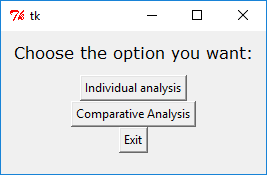
\includegraphics[width=6cm, height=4cm]{VentanaPrincipal}
\caption{Vista de la ventana principal}
\end{figure}

En el caso de querer ver el porcentaje de eficiencia que proporciona cada tipo de operación de un fichero, el análisis individual es la opción adecuada.
Por otra parte si lo que se quiere es hacer una comparación de eficiencia entre ficheros, el análisis Múltiple es el que debes pulsar.


\subsection{Análisis individual}

Si pulsamos el análisis individual, lo primero que nos saldrá será una ventana con dos botones, buscar fichero y volver a la ventana principal.\\
\begin{figure}[H]
\centering
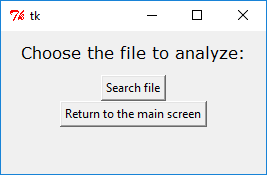
\includegraphics[width=6cm, height=4cm]{VentanaIntermedia}
\caption{Vista de la ventana principal}
\end{figure}
El primero de estos nos permite buscar el fichero que deseamos analizar a través de un explorador de archivos, el archivo seleccionado debe tener un formato.py, ya que si no nos saldrá un mensaje de error indicando que es un tipo de formato no válido.\\
\begin{figure}[H]
\centering
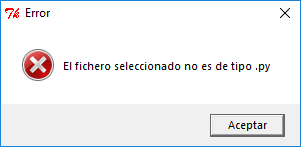
\includegraphics[width=5cm, height=3cm]{Error}
\caption{Mensaje de error}
\end{figure}
Algo parecido aparecerá si no elegimos ningún fichero, como advertencia saldrá  también un mensaje\\
\begin{figure}[H]
\centering
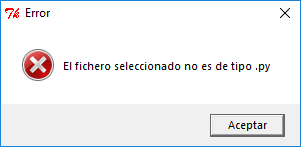
\includegraphics[width=5cm, height=3cm]{Error}
\caption{Mensaje de advertencia}
\end{figure}
Si por el contrario pulsamos el botón de volver a la ventana principal, esto hará que aparezca de nuevo la ventana que se mostró al principio.\\

Una vez seleccionado el archivo .py aparecerá un nuevo botón en el que pondrá analizar fichero. A veces puede que tarde un poco en mostrar el fichero, porque internamente la herramienta tiene que hacer una serie de cálculos.\\
\begin{figure}[H]
\centering
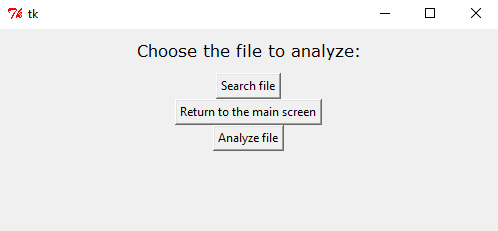
\includegraphics[width=6cm, height=4cm]{VentanaIntermedia2}
\caption{Aparición del botón tras la elección de un archivo .py}
\end{figure}
Si pulsamos ese botón, nos mostrará la ventana de análisis. En esta ventana se muestran los resultados del análisis hecho al fichero que ha sido elegido en la ventana previa. Cuenta con una serie de opciones que hará variar los resultados que serán mostrados.\\

Echando un vistazo de arriba abajo nos encontramos con las siguientes opciones:\\

\begin{enumerate}
	\item Primero al igual que en la ventana anterior a esta, nos encontramos con un botón que nos deja volver a la ventana inicial. Por si queremos realizar algún tipo de análisis más.\\

	\item Despues hay un boton que nos lleva a otra ventana donde se pueden ver unos checkboxes que representan los diferentes tipos de operaciones encontrados en el análisis del fichero seleccionado, que por defecto al principio saldrán todos marcados. Esto indica que operaciones van a ser mostradas en la gráfica de los resultados, si hay algún tipo de operación que no queramos que salga tan solo tendríamos que clicar en el checkbox de la operación para quitarle la marca. Cuando queden marcadas aquellas operaciones que deseemos hay un boton para volver a la vista anterior en la parte de abajo.\\

\begin{figure}[H]
\centering
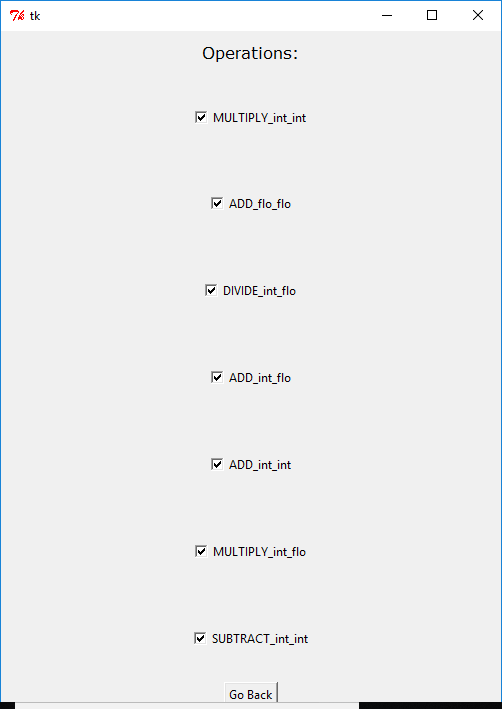
\includegraphics[width=6cm, height=7cm]{Operaciones}
\caption{Ventana donde elegir operaciones}
\end{figure}

	\item Seguido a esto hay una Listbox que deja elegir el procesador con el que se quiere ponderar a las operaciones. En esta lista se muestran los procesadores que tengamos disponibles en la carpeta Prueba TFG. Así que si queremos que aparezcan mas tipos de procesadores tan solo habría que crear más procesadores teóricos ahí.\\

(Se recomienda copiar un procesador ya creado y tan solo tener que cambiar los valores según se desee)\\

\begin{figure}[H]
\centering
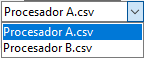
\includegraphics[width=4cm, height=2cm]{ListBox}
\caption{Ejemplo de la Listbox de procesadores}
\end{figure}

	\item Una vez configurados todos estos valores anteriores, habría que pulsar el botón de abajo Mostrar resultados, y tras esto saldría la gráfica resultante.\\
\begin{figure}[H]
\centering
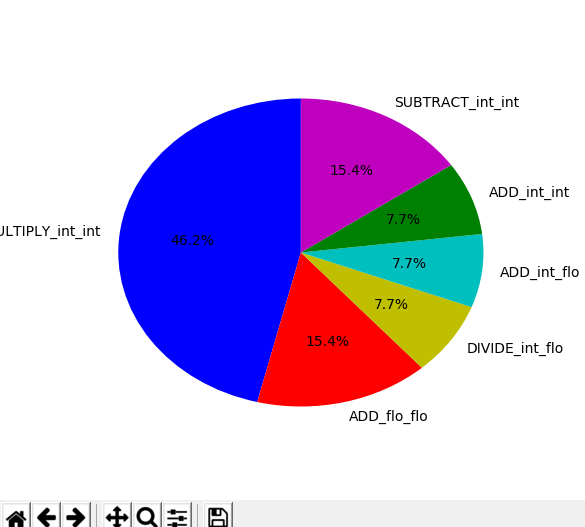
\includegraphics[width=8cm, height=7cm]{Grafica2}
\caption{Ejemplo gráfica resultante análisis individual}
\end{figure}
	\item Hay que tener en cuenta que la configuración puede ser cambiada aunque ya se haya mostrado una gráfica y si se vuelve a pulsar el botón mostrar resultados, vuelve a recargar la gráfica con la nueva configuración que haya sido elegida.\\

\begin{figure}[H]
\centering
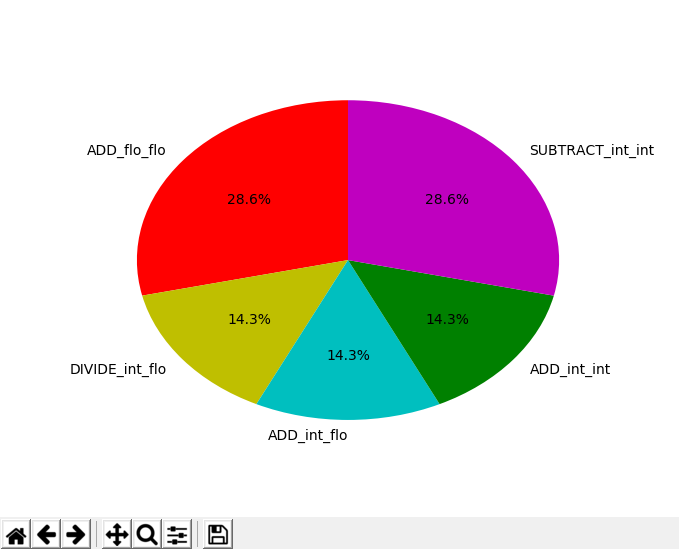
\includegraphics[width=8cm, height=7cm]{Grafica3}
\caption{Ejemplo gráfica resultante recalculada}
\end{figure}

\end{enumerate}

En este caso se ha quitado la marca de la multiplicación de enteros y vemos como este desaparece de la gráfica. Esto mismo se podría hacer también con la listbox de los procesadores.

La gráfica muestra los porcentajes de ciclos de reloj que consume cada tipo de operación. Cada uno diferenciado por un color e indicado con el nombre de la operación y el nombre del tipo de los dos operadores.

Como se puede ver en la última imagen en la parte de abajo hay una serie de botones que nos permiten hacer un par de interacciones con el gráfico como por ejemplo ampliar la zona deseada o poder guardarla.

\subsection{Análisis Múltiple}
Pulsando el botón de análisis Múltiple, Muestra una ventana con dos tipos de opciones, Buscar ficheros y volver a la ventana inicial. Esta ventana es prácticamente idéntica a la primera que sale en el análisis individual (Figura B2). Pero la diferencia que hay en esta se trata del botón buscar ficheros, con el cual sale un explorador de archivos pero con el que hay que seleccionar mas de un fichero. Al igual que en el análisis individual solo se pueden elegir ficheros con formato .py pero además no se puede elegir solo 1 fichero, ya que se hace alguna de estas dos cosas saldrá un mensaje de error.\\

\begin{figure}[H]
\centering
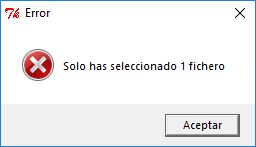
\includegraphics[width=5cm, height=3cm]{Error2}
\caption{Mensaje de error por elegir solo un fichero}
\end{figure}

Una vez seleccionado el fichero saldrá el botón de Analizar, y este nos pasará a la ventana de análisis.\\
Lo primero que vemos en la ventana de análisis es el botón de volver al menú principal en caso de que deseemos hacer el otro tipo de análisis o el mismo con otros ficheros.\\

Seguido hay una listbox que para indicar el procesador teórico con el que se desea ponderar  las operaciones sacadas por el intérprete.\\
Seguido a esto hay un botón que nos lleva a otra ventana donde hay una serie de checkboxes, pero a diferencia del análisis individual, aquí muestra todas las diferentes operaciones que aparecen en todos los ficheros. Así que puede haber operaciones del checkbox que se encuentren solo en un fichero.\\
Una vez elegidos los parámetros está el botón mostrar resultados que nos muestra la gráfica resultante, según los parámetros establecidos. La gráfica se  puede volver a recalcular sin salirse de la ventana volviendo a  pulsar el botón de mostrar resultados y mostrara la gráfica según como estén los parámetros.\\

La gráfica muestra los ciclos de reloj totales que suman todas las operaciones en cada uno de los ficheros seleccionados, a través de una gráfica de barras, si se han seleccionado menos de 10 ficheros y en caso contrario, a través de un gráfico de puntos. Los nombres de los ficheros en la gráfica son sustituidos por letras en orden alfabético. Y como se ha indicado antes para ver el nombre de cada uno hay que buscar en la celda de texto que fichero está asociado a cada nombre.\\

\begin{figure}[H]
\centering
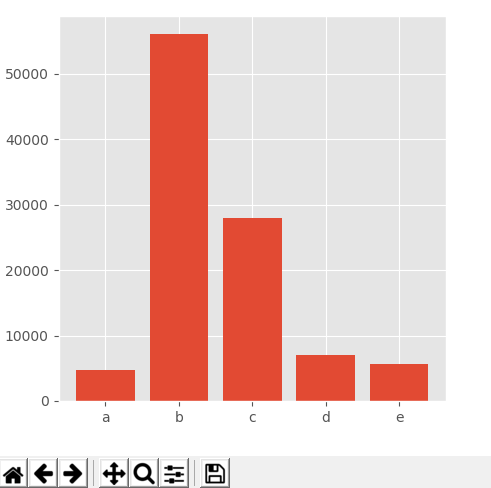
\includegraphics[width=9cm, height=10cm]{Grafica5}
\caption{Gráfico de barras resultante}
\end{figure}

\begin{figure}[H]
\centering
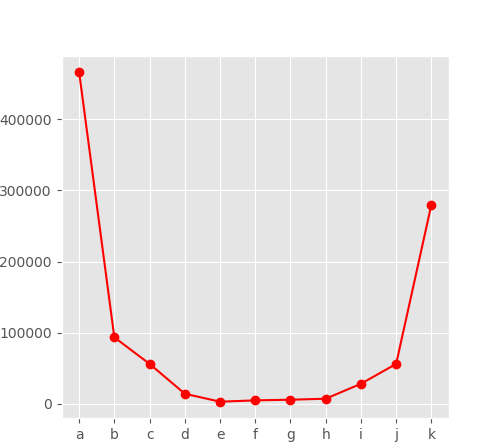
\includegraphics[width=9cm, height=10cm]{Grafica6}
\caption{Gráfico de puntos resultante}
\end{figure}



